\lecture_date{03/11/2026}
\chapter{Lecture 07}

\section{Multivariate optimality conditions}
\label{sec:lec07-optimality}
Last time, we used the multivariable chain rule to calculate directional derivatives, and introduced the gradient, Hessian and Taylor expansion. We now put these ideas together to classify stationary points. Throughout this section, $U\subseteq\mathbb{R}^n$ is open. We study unconstrained extrema at interior points of $U$; boundary points require a separate analysis.

\subsection{A short review: directional derivatives and the gradient}
For a differentiable function $f:U\to\mathbb{R}$, a point $x_0\in U$ and a vector $v\in\mathbb{R}^n$, recall that
\begin{equation}
 D_vf(x_0)=\lim_{t\to0}\frac{f(x_0+tv)-f(x_0)}{t}
 =\sum_{i=1}^n v_i\frac{\partial f}{\partial x_i}(x_0)
 =\langle\nabla f(x_0),v\rangle.
 \label{eq:lec07-directional}
\end{equation}
Here the gradient is the column vector
\[
 \nabla f(x_0)=\begin{bmatrix}
 \frac{\partial f}{\partial x_1}(x_0)\\ \vdots\\
 \frac{\partial f}{\partial x_n}(x_0)
 \end{bmatrix}\in\mathbb{R}^n.
\]
The gradient is a vector, whereas the directional derivative is a scalar. Once we know the gradient at a point, we can calculate the derivative along any chosen direction by taking an inner product.

Here $v$ need not be a unit vector: it specifies the direction and speed along $x_0+tv$, as in the lecture.

\subsection{The Hessian and second-order change}
\begin{definition}[Hessian matrix]
Let $f\in C^2(U)$, meaning that its partial derivatives up to order two are continuous. Its Hessian at $x$ is the $n\times n$ matrix
\begin{equation}
 H_f(x)=\nabla^2f(x)
 =\left[\frac{\partial}{\partial x_i}
       \left(\frac{\partial f}{\partial x_j}\right)(x)\right]_{i,j=1}^n.
 \label{eq:lec07-hessian}
\end{equation}
For two variables, this is
\[
 H_f(x)=\begin{bmatrix}
 \frac{\partial^2f}{\partial x_1^2}(x)&
 \frac{\partial^2f}{\partial x_1\partial x_2}(x)\\[5pt]
 \frac{\partial^2f}{\partial x_2\partial x_1}(x)&
 \frac{\partial^2f}{\partial x_2^2}(x)
 \end{bmatrix}.
\]
\end{definition}
The entry in row $i$, column $j$ differentiates first with respect to $x_j$, then with respect to $x_i$. Since $f\in C^2(U)$, the mixed partial derivatives agree. Consequently,
\[
 H_f(x)^T=H_f(x).
\]
Thus the Hessian is real symmetric and has real eigenvalues and an orthonormal eigenbasis.

For a displacement $h\in\mathbb{R}^n$, the scalar
\begin{equation}
 h^TH_f(x_0)h
 =\sum_{i=1}^n\sum_{j=1}^n h_i h_j
    \frac{\partial^2 f}{\partial x_i\partial x_j}(x_0)
 =\langle h,H_f(x_0)h\rangle
 \label{eq:lec07-quadratic}
\end{equation}
is a \emph{quadratic form}. It describes the second-order change of $f$ near $x_0$.

\subsection{Multivariable Taylor expansion}
\begin{theorem}[Second-order Taylor expansion]
If $f\in C^2(U)$ and $x_0\in U$, then, as $h\to0$,
\begin{equation}
 f(x_0+h)=f(x_0)+\nabla f(x_0)^Th
       +\frac12 h^TH_f(x_0)h+r(h),
 \qquad r(h)=o(\|h\|^2).
 \label{eq:lec07-taylor}
\end{equation}
The remainder notation means $r(h)/\|h\|^2\to0$ as $h\to0$, $h\ne0$.
\end{theorem}

In two variables, the quadratic term is
\[
 \frac12\left(h_1^2 f_{11}(x_0)
 +2h_1h_2 f_{12}(x_0)+h_2^2 f_{22}(x_0)\right),
 \qquad f_{ij}=\frac{\partial^2 f}{\partial x_i\partial x_j}.
\]
The mixed term is essential. A quadratic form need not be positive just because it has degree two.

The next Taylor term mentioned in class is
\[
 \frac{1}{3!}\sum_{i,j,k=1}^n
 h_i h_j h_k\frac{\partial^3f}{\partial x_i\partial x_j\partial x_k}(x_0).
\]
These derivatives have three indices and form a third-order tensor. Higher-order terms become more complicated, so we will use the test up to order two.

\subsection{First-order necessary condition}
At a local minimum $x_0$, there is a neighbourhood in which
\[
 \Delta f=f(x_0+h)-f(x_0)\ge0.
\]
At a local maximum, the inequality is reversed. For a strict extremum, the corresponding inequality is strict for sufficiently small nonzero $h$.

\begin{proposition}[First-order necessary condition]
If $f$ is differentiable at an interior local minimum or maximum $x_0$, then
\begin{equation}
 \nabla f(x_0)=0.
 \label{eq:lec07-first-order}
\end{equation}
\end{proposition}
\begin{proof}
Fix any $v\in\mathbb{R}^n$ and consider $g(t)=f(x_0+tv)$ for sufficiently small positive and negative $t$. The function $g$ has a local extremum at zero, so
\[
 0=g'(0)=\nabla f(x_0)^Tv.
\]
This holds for every $v$. Taking $v=\nabla f(x_0)$ gives $\|\nabla f(x_0)\|^2=0$.
\end{proof}
A point where $\nabla f(x_0)=0$ is called a \emph{stationary point} (or a critical point in our differentiable setting). It is a candidate for an extremum, not necessarily an extremum. Finding such points means solving
\[
 \frac{\partial f}{\partial x_1}=0,\quad\ldots,\quad
 \frac{\partial f}{\partial x_n}=0.
\]
This system can have no solutions, one solution, several solutions or infinitely many solutions.

\subsection{Quadratic forms and eigenvalues}
Let $H$ be a real symmetric matrix. Choose an orthonormal eigenbasis $q_1,\ldots,q_n$, with $Hq_i=\lambda_iq_i$. Every $h$ has a unique expansion $h=\sum_i a_iq_i$. Then
\begin{equation}
 Hh=\sum_i a_i\lambda_iq_i,
 \qquad h^THh=\sum_{i,j}a_i a_j\lambda_j\langle q_i,q_j\rangle
             =\sum_{i=1}^n\lambda_i a_i^2.
 \label{eq:lec07-spectral}
\end{equation}
Since $\langle q_i,q_j\rangle=\delta_{ij}$, the cross terms vanish in this basis. We obtain the following classification.
\begin{center}
\small
\begin{tabular}{lll}
\toprule
Type of $H$ & Quadratic form, for every $h\ne0$ & Eigenvalues\\
\midrule
Positive definite (PD) & $h^THh>0$ & All $\lambda_i>0$\\
Negative definite (ND) & $h^THh<0$ & All $\lambda_i<0$\\
Positive semidefinite (PSD) & $h^THh\ge0$ & All $\lambda_i\ge0$\\
Negative semidefinite (NSD) & $h^THh\le0$ & All $\lambda_i\le0$\\
Indefinite & Takes both positive and negative values & Both signs occur\\
\bottomrule
\end{tabular}
\end{center}
Positive definite matrices are also positive semidefinite. When a semidefinite matrix has a zero eigenvalue, it is singular and is not definite.

Geometrically, $h^THh=\langle h,Hh\rangle$. If $H$ is PD, the angle between $h$ and $Hh$ is acute for every nonzero $h$; if $H$ is ND, it is obtuse. The transformation can change both length and direction. It need not keep $Hh$ parallel to $h$.

\subsection{Second-order necessary and sufficient conditions}
\begin{proposition}[Second-order necessary condition]
Let $f\in C^2(U)$. If $x_0$ is a local minimum, then $\nabla f(x_0)=0$ and $H_f(x_0)$ is PSD. If $x_0$ is a local maximum, then $\nabla f(x_0)=0$ and $H_f(x_0)$ is NSD.
\end{proposition}
\begin{proof}
At a local minimum, $g(t)=f(x_0+tv)$ has a local minimum at zero. Thus $g''(0)=v^TH_f(x_0)v\ge0$ for every $v$. This is precisely positive semidefiniteness. Apply the same argument to $-f$ for a maximum.
\end{proof}

\begin{theorem}[Second-order classification of stationary points]
\label{thm:lec07-classification}
Let $f\in C^2(U)$ and suppose $\nabla f(x_0)=0$.
\begin{enumerate}
 \item If $H_f(x_0)$ is PD, then $x_0$ is a strict local minimum.
 \item If $H_f(x_0)$ is ND, then $x_0$ is a strict local maximum.
 \item If $H_f(x_0)$ is indefinite, then $x_0$ is a saddle point: every neighbourhood contains points with values larger and smaller than $f(x_0)$.
 \item If $H_f(x_0)$ is singular PSD or singular NSD, the second-order test is inconclusive.
\end{enumerate}
\end{theorem}
To understand the test, at a stationary point Taylor expansion gives
\[
 f(x_0+h)-f(x_0)=\frac12h^TH_f(x_0)h+o(\|h\|^2).
\]
If the Hessian is PD, the positive quadratic term controls the sign for all sufficiently small nonzero displacements, giving a strict local minimum. The ND case gives a strict local maximum. If the Hessian is indefinite, positive and negative eigenvalues give directions in which the function increases and decreases, so the point is a saddle. In the singular semidefinite case, the quadratic term vanishes in some directions, and higher-order terms may decide the result.

\begin{example}[Why semidefinite is inconclusive]
At the origin, both $f_+(x,y)=x^2+y^4$ and $f_-(x,y)=x^2-y^4$ have zero gradient and Hessian
\[
 \begin{bmatrix}2&0\\0&0\end{bmatrix}.
\]
Yet $f_+$ has a strict global minimum there, while $f_-$ has a saddle point: $f_-(t,0)>0$ and $f_-(0,t)<0$ for $t\ne0$. Thus PD is sufficient but not necessary for a strict minimum, and PSD alone is not sufficient. Negating these examples gives the corresponding NSD cases.
\end{example}
A zero eigenvalue means that the quadratic term vanishes in that direction; higher-order change may still occur. When considering higher-order tests, it is the \emph{first nonzero} Taylor term that matters: a leading odd-degree term rules out a local extremum.

\begin{example}[Finishing the Lecture 06 stationary-point example]
For $f(x_1,x_2)=x_1^2+3x_1x_2$, the only stationary point is $(0,0)$ and
\[
 H_f=\begin{bmatrix}2&3\\3&0\end{bmatrix},
 \qquad \det(H_f-\lambda I)=\lambda^2-2\lambda-9.
\]
The eigenvalues $1\pm\sqrt{10}$ have opposite signs. Therefore $(0,0)$ is a saddle point. Directly, $f(t,0)=t^2>0$, whereas $f(t,-t)=-2t^2<0$ for $t\ne0$.
\end{example}

\clearpage
\section{A worked example: the Rosenbrock function}
\label{sec:lec07-rosenbrock}
\begin{example}
Consider the Rosenbrock-type function
\begin{equation}
 f(x_1,x_2)=(1-x_1)^2+5(x_2-x_1^2)^2,
 \qquad (x_1,x_2)\in\mathbb{R}^2.
 \label{eq:lec07-rosenbrock}
\end{equation}
\begin{enumerate}
 \item Calculate $D_vf(x_0)$ at $x_0=(1,2)^T$ for $v=(2,-3)^T$.
 \item Find and classify all stationary points.
\end{enumerate}
\end{example}
The function is often called a banana function because of its curved level sets. We first differentiate symbolically and only then substitute the point of interest.

\subsection{Gradient and directional derivative}
Using the chain rule,
\begin{align*}
 \frac{\partial f}{\partial x_1}
 &=2(1-x_1)(-1)+5\cdot2(x_2-x_1^2)(-2x_1)\\
 &=-2(1-x_1)-20x_1(x_2-x_1^2),\\
 \frac{\partial f}{\partial x_2}
 &=5\cdot2(x_2-x_1^2)\cdot1=10(x_2-x_1^2).
\end{align*}
Therefore,
\begin{equation}
 \nabla f(x_1,x_2)=\begin{bmatrix}
 -2(1-x_1)-20x_1(x_2-x_1^2)\\
 10(x_2-x_1^2)
 \end{bmatrix}.
 \label{eq:lec07-rosenbrock-gradient}
\end{equation}
At the specified point $x_0=(1,2)^T$,
\[
 \nabla f(1,2)=\begin{bmatrix}-20\\10\end{bmatrix},
 \qquad
 D_vf(1,2)=\left\langle\begin{bmatrix}-20\\10\end{bmatrix},
 \begin{bmatrix}2\\-3\end{bmatrix}\right\rangle
 =-40-30=\boxed{-70}.
\]
The negative directional derivative means that moving a sufficiently small positive amount along $v$ decreases the function value.

\subsection{Finding the stationary point}
Set \autoref{eq:lec07-rosenbrock-gradient} equal to zero:
\[
 \begin{cases}
 -2(1-x_1)-20x_1(x_2-x_1^2)=0,\\
 10(x_2-x_1^2)=0.
 \end{cases}
\]
The second equation gives $x_2=x_1^2$. Substituting this into the first equation eliminates the product term:
\[
 -2(1-x_1)=0\quad\Longrightarrow\quad x_1=1,
 \qquad x_2=1.
\]
Hence $x^*=(1,1)^T$ is the unique stationary point. At this stage we have found a candidate, and must still classify it.

\subsection{Hessian and classification}
Differentiate the first partial derivatives once more:
\begin{align*}
 f_{11}&=\frac{\partial}{\partial x_1}
       (-2+2x_1-20x_1x_2+20x_1^3)
       =2-20x_2+60x_1^2,\\
 f_{12}&=\frac{\partial}{\partial x_1}\bigl(10(x_2-x_1^2)\bigr)
       =-20x_1,\\
 f_{21}&=\frac{\partial}{\partial x_2}
       \bigl(-2(1-x_1)-20x_1(x_2-x_1^2)\bigr)=-20x_1,\\
 f_{22}&=\frac{\partial}{\partial x_2}\bigl(10(x_2-x_1^2)\bigr)=10.
\end{align*}
The mixed derivatives agree, as expected. Therefore,
\begin{equation}
 H_f(x_1,x_2)=\begin{bmatrix}
 2-20x_2+60x_1^2&-20x_1\\-20x_1&10
 \end{bmatrix},
 \qquad H_f(1,1)=\begin{bmatrix}42&-20\\-20&10\end{bmatrix}.
 \label{eq:lec07-rosenbrock-hessian}
\end{equation}
Notice that the Hessian is evaluated at the stationary point $(1,1)$, not the directional-derivative point $(1,2)$.

To find the eigenvalues, solve
\begin{align*}
 0=\det(H_f(1,1)-\lambda I)
 &=(42-\lambda)(10-\lambda)-400\\
 &=\lambda^2-52\lambda+20.
\end{align*}
Thus
\begin{equation}
 \lambda_{\pm}=\frac{52\pm\sqrt{2704-80}}{2}
 =26\pm2\sqrt{164}
 \approx 51.612497,  0.387503.
 \label{eq:lec07-rosenbrock-eigenvalues}
\end{equation}
Both eigenvalues are positive: $0<\sqrt{2624}<52$. Hence the Hessian is PD and $x^*=(1,1)^T$ is a strict local minimum.

\subsection{Is the minimum global?}
The Hessian test establishes only a local conclusion. For this particular function, we can establish a stronger result directly:
\[
 f(x_1,x_2)=(1-x_1)^2+5(x_2-x_1^2)^2\ge0
 \qquad\text{for all }(x_1,x_2)\in\mathbb{R}^2.
\]
Equality holds exactly when both squares vanish:
\[
 1-x_1=0,\qquad x_2-x_1^2=0
 \quad\Longleftrightarrow\quad (x_1,x_2)=(1,1).
\]
Therefore $(1,1)$ is the \emph{unique global minimiser}, and the global minimum value is $f(1,1)=0$. This short observation strengthens the local conclusion obtained in class.

There are no other stationary points, so there are no local maxima or stationary saddle points. There is no global maximum either, since $f(1,x_2)=5(x_2-1)^2\to\infty$ as $|x_2|\to\infty$.

\paragraph{Calculation procedure.}
For an unconstrained $C^2$ objective on an open domain:
\begin{enumerate}
 \item Calculate the gradient and solve $\nabla f(x)=0$ for all stationary points.
 \item Calculate the Hessian symbolically, then evaluate it at each stationary point.
 \item Classify using its eigenvalue signs: PD gives a strict local minimum, ND gives a strict local maximum, and indefinite gives a saddle point. A singular semidefinite Hessian leaves the test inconclusive.
 \item Distinguish local conclusions from global ones. A global claim needs an additional argument, such as the nonnegative-square decomposition above.
\end{enumerate}


% Appended continuation: Lecture 07 numerical differentiation.
% Sources: supplied differentiation transcript (from 50:28) and four whiteboards.
% The uploaded prefix above is preserved byte-for-byte.
\clearpage
\section{Differentiation}
\label{sec:lec07-differentiation}
So far, we have calculated derivatives by writing down exact formulas. In optimisation, however, we often need the value of a derivative at a particular point, and the function may be given as a computer program. How can we calculate these derivatives?

\subsection{Symbolic, numerical and automatic differentiation}
The lecture distinguishes three approaches.
\begin{enumerate}
 \item \emph{Symbolic differentiation} manipulates expressions using known derivative formulas, the product rule and the chain rule. This gives a formula for the derivative, as in our Rosenbrock example. For complicated functions, the resulting expressions can become large and expensive to store or evaluate.
 \item \emph{Numerical differentiation} estimates derivatives using function values. The formulas themselves generally introduce an approximation error, even if all arithmetic were exact. On a computer, rounding error is present as well.
 \item \emph{Automatic differentiation} applies the chain rule through the elementary operations of a computation, often represented by a computational graph. It calculates derivative values without constructing a large symbolic expression or taking finite differences. For differentiable operations, there is no finite-difference truncation error; floating-point rounding error still remains. We will study this approach later.
\end{enumerate}
The numerical methods listed in class are forward difference, backward difference, central difference, complex step and stochastic methods. The discussion develops the first four; stochastic methods are only mentioned here.

\subsection{Forward, backward and central differences}
For now, consider a single-variable function $f:\mathbb{R}\to\mathbb{R}$. We want $f'(x_0)$ and can evaluate $f$ at nearby points. Choose a small \emph{nonzero} step $h>0$, with the required points in the domain.
\begin{definition}[Finite-difference approximations]
The forward, backward and central differences are, respectively,
\begin{align}
 \operatorname{FD}_h f(x_0)&=\frac{f(x_0+h)-f(x_0)}{h},
 \label{eq:lec07-fd}\\
 \operatorname{BD}_h f(x_0)&=\frac{f(x_0)-f(x_0-h)}{h},
 \label{eq:lec07-bd}\\
 \operatorname{CD}_h f(x_0)&=\frac{f(x_0+h)-f(x_0-h)}{2h}.
 \label{eq:lec07-cd}
\end{align}
\end{definition}
Geometrically, these are slopes of secant lines approximating the tangent at $x_0$. Forward difference looks to the right, backward difference to the left, and central difference uses points on both sides. The central denominator is $2h$ because that is the distance between its two sample points.


\begin{center}
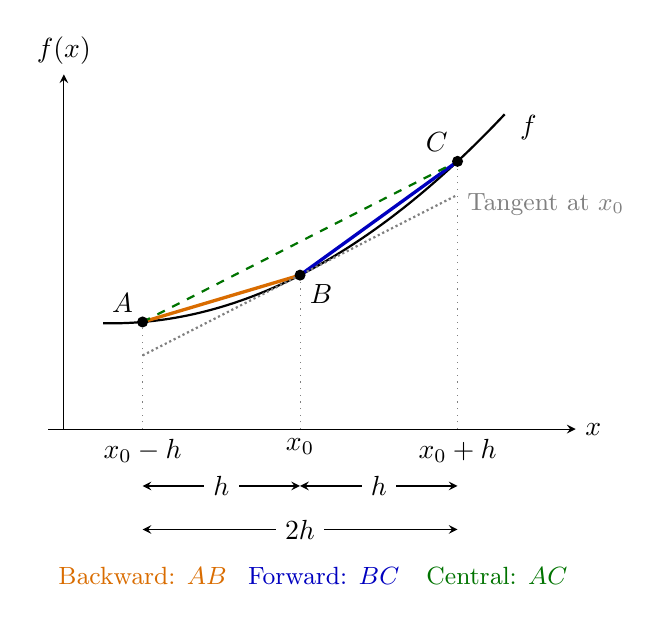
\begin{tikzpicture}[x=1cm,y=0.85cm,>=stealth]
 \draw[->] (0.8,0) -- (7.5,0) node[right] {$x$};
 \draw[->] (1,0) -- (1,5.3) node[above] {$f(x)$};
 \draw[thick,domain=1.5:6.6,samples=80]
   plot (\x,{0.5*((\x-4)/2)^2+1.2*((\x-4)/2)+2.3});
 \node at (6.9,4.5) {$f$};
 % Secants join the exact sample points on the curve.
 \draw[very thick,orange!85!black] (2,1.6) -- (4,2.3);
 \draw[very thick,blue!75!black] (4,2.3) -- (6,4);
 \draw[thick,dashed,green!45!black] (2,1.6) -- (6,4);
 \draw[gray,densely dotted,thick] (2,1.1) -- (6,3.5);
 \node[gray,right,font=\small] at (6,3.35) {Tangent at $x_0$};
 \foreach \x/\y/\lab in {2/1.6/{x_0-h},4/2.3/{x_0},6/4/{x_0+h}} {
  \draw[dotted,gray] (\x,0) -- (\x,\y);
  \fill (\x,\y) circle (2pt);
  \node[below] at (\x,0) {$\lab$};
 }
 \node[above left] at (2,1.6) {$A$};
 \node[below right] at (4,2.3) {$B$};
 \node[above left] at (6,4) {$C$};
 \draw[<->] (2,-0.85) -- (4,-0.85) node[midway,fill=white] {$h$};
 \draw[<->] (4,-0.85) -- (6,-0.85) node[midway,fill=white] {$h$};
 \draw[<->] (2,-1.5) -- (6,-1.5) node[midway,fill=white] {$2h$};
 \node[orange!85!black,font=\small] at (2,-2.2) {Backward: $AB$};
 \node[blue!75!black,font=\small] at (4.3,-2.2) {Forward: $BC$};
 \node[green!45!black,font=\small] at (6.5,-2.2) {Central: $AC$};
\end{tikzpicture}

\small Each approximation is rise divided by run along its secant.
\end{center}
The central secant joins $A$ to $C$; it need not pass through $B$. Its horizontal run is $2h$, whereas the other two runs are $h$. The dotted tangent shows the derivative we want to approximate.

If $f$ is differentiable at $x_0$, all three converge to $f'(x_0)$ as $h\to0$ in exact arithmetic. In an actual calculation, we use a finite $h$, so the result is generally only approximate. Each formula uses two function evaluations when neither value is already available.

\subsection{Taylor expansion and approximation error}
Taylor expansion tells us how the error depends on $h$. Assume $f\in C^3$ in a neighbourhood of $x_0$. Then
\begin{align}
 f(x_0+h)&=f(x_0)+hf'(x_0)+\frac{h^2}{2}f''(x_0)+O(h^3),
 \label{eq:lec07-taylor-plus}\\
 f(x_0-h)&=f(x_0)-hf'(x_0)+\frac{h^2}{2}f''(x_0)+O(h^3).
 \label{eq:lec07-taylor-minus}
\end{align}
Here $O(h^p)$ means that the remainder is bounded in magnitude by a constant times $|h|^p$ for small $h$. This differs from $o(h^p)$, which means the remainder divided by $h^p$ tends to zero. We use $O(h^3)$ above: the omitted cubic term is generally not $o(h^3)$.

\paragraph{Forward and backward differences.}
Subtract $f(x_0)$ from \autoref{eq:lec07-taylor-plus} and divide by $h$:
\begin{equation}
 \operatorname{FD}_h f(x_0)
 =f'(x_0)+\frac{h}{2}f''(x_0)+O(h^2)
 =f'(x_0)+O(h).
 \label{eq:lec07-fd-error}
\end{equation}
Similarly, rearranging \autoref{eq:lec07-taylor-minus} gives
\begin{equation}
 \operatorname{BD}_h f(x_0)
 =f'(x_0)-\frac{h}{2}f''(x_0)+O(h^2)
 =f'(x_0)+O(h).
 \label{eq:lec07-bd-error}
\end{equation}
Thus both methods have \emph{first-order} truncation error. Their leading errors have opposite signs, but the same order in $h$.

\paragraph{Central difference.}
Subtract the two Taylor expansions. The constant and quadratic terms cancel:
\[
 f(x_0+h)-f(x_0-h)=2hf'(x_0)+O(h^3).
\]
Dividing by $2h$ gives
\begin{equation}
 \operatorname{CD}_h f(x_0)=f'(x_0)+O(h^2).
 \label{eq:lec07-cd-error}
\end{equation}
Central difference therefore has \emph{second-order} truncation error, while still using two function evaluations. When truncation error dominates and the leading coefficient is nonzero, halving $h$ roughly halves the forward or backward error, but reduces the central error by a factor of four.

\subsection{Why not choose an extremely small step?}
The errors above come from replacing a derivative by a finite-step formula. This is \emph{truncation error}. It decreases as $h$ decreases. A computer introduces another issue: function values and arithmetic are stored with finite precision.

When $h$ is very small, $f(x_0+h)$ and $f(x_0)$ can be almost equal. Their subtraction cancels the shared leading digits, leaving a small difference in which errors already present in the function values can be significant. Dividing by the small number $h$ then amplifies these errors. This is the cancellation problem discussed in class. Eventually, $x_0+h$ may even round to $x_0$, or the two computed function values may become identical. The computed derivative can then be zero rather than the correct value.

In short, the total error has two competing contributions: truncation decreases with $h$, while rounding errors in the function values can be amplified by division by $h$. This explains the following overall trend.

\begin{center}
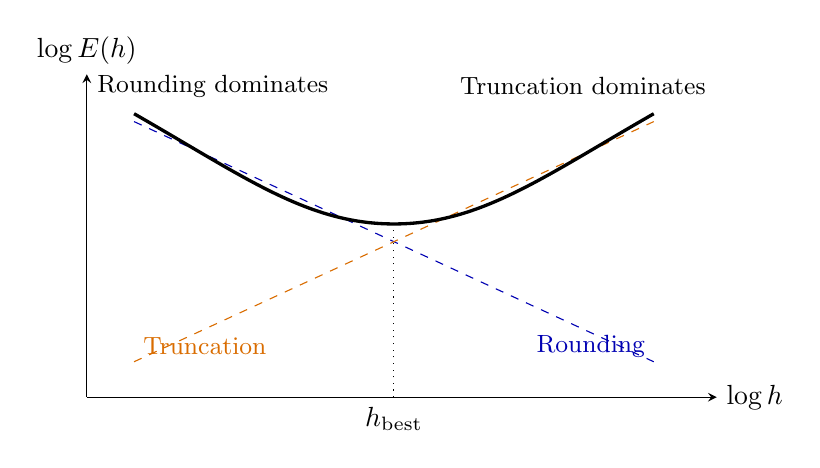
\begin{tikzpicture}[x=1cm,y=1cm,>=stealth]
 \draw[->] (0,0) -- (8,0) node[right] {$\log h$};
 \draw[->] (0,0) -- (0,4.1) node[above] {$\log E(h)$};
 \draw[dashed,blue!70!black] (0.6,3.5) -- (7.2,0.45);
 \draw[dashed,orange!85!black] (0.6,0.45) -- (7.2,3.5);
 \draw[very thick] (0.6,3.6) .. controls (2.0,2.8) and (2.8,2.2) .. (3.9,2.2)
   .. controls (5.0,2.2) and (5.8,2.8) .. (7.2,3.6);
 \draw[dotted] (3.9,0) -- (3.9,2.2);
 \node[below] at (3.9,0) {$h_{\mathrm{best}}$};
 \node[align=center,font=\small] at (1.6,3.95) {Rounding dominates};
 \node[align=center,font=\small] at (6.3,3.95) {Truncation dominates};
 \node[blue!70!black,font=\small] at (6.4,0.65) {Rounding};
 \node[orange!85!black,font=\small] at (1.5,0.65) {Truncation};
\end{tikzpicture}

\small Schematic log--log error plot. The solid curve shows the combined trend.
\end{center}
Starting from a large step and decreasing $h$, the error usually decreases until rounding becomes important, then increases or behaves irregularly. The measured curve need not be perfectly smooth. Thus $h\to0$ is correct in the mathematical limit, but is not always the best numerical strategy at fixed precision.

\subsection{Choosing the step size}
The lecture uses the order of the error to estimate a suitable step. For example, ignoring constants and rounding, an $O(h^2)$ error suggests $h\approx10^{-2}$ for an error scale of $10^{-4}$. For a scale of $10^{-5}$, the corresponding estimate is $h\approx10^{-2.5}$; taking $h=10^{-3}$ gives $h^2=10^{-6}$. Fractional powers are perfectly valid choices.

These are estimates, not guarantees: $O(h^2)$ does not mean the error equals $h^2$ or is bounded by $h^2$ with constant one. The derivatives hidden in the constant and the rounding error also matter.

Choose $h$ according to the required accuracy and the scale of the problem, and compare the estimates for a few decreasing step sizes. Stop shrinking the step once rounding prevents further improvement.

\subsection{The complex-step method}
Can we avoid subtracting nearly equal function values? The complex-step method separates the derivative information into the imaginary component.

Assume that our real-valued function has an analytic extension to a complex neighbourhood of $x_0$, agreeing with $f$ on the real axis. We use the same symbol $f$ for this extension. Its Taylor expansion is valid for sufficiently small complex steps. With $i^2=-1$,
\begin{align*}
 f(x_0+ih)
 &=f(x_0)+ihf'(x_0)-\frac{h^2}{2!}f''(x_0)
   -i\frac{h^3}{3!}f'''(x_0)\\
 &\qquad+\frac{h^4}{4!}f^{(4)}(x_0)+O(h^5).
\end{align*}
Since the derivatives at $x_0$ are real, the even-power terms shown are real and the odd-power terms are imaginary. Recall that $\operatorname{Im}(a+ib)=b$, not $ib$. Taking imaginary parts gives
\[
 \operatorname{Im}f(x_0+ih)
 =hf'(x_0)-\frac{h^3}{6}f'''(x_0)+O(h^5).
\]
Divide by the real, nonzero step $h$:
\begin{equation}
 \frac{\operatorname{Im}f(x_0+ih)}{h}
 =f'(x_0)-\frac{h^2}{6}f'''(x_0)+O(h^4)
 =f'(x_0)+O(h^2).
 \label{eq:lec07-complex-step}
\end{equation}
Thus the complex-step approximation is
\[
 \boxed{f'(x_0)\approx\frac{\operatorname{Im}f(x_0+ih)}{h}.}
\]
It has second-order truncation error, like central difference, and uses one complex function evaluation.

\paragraph{Why this helps.}
There is no subtraction of two nearby function values. The real baseline $f(x_0)$ does not enter the imaginary component. With an implementation that accurately carries the small imaginary perturbation, we can often choose a much smaller $h$ than with ordinary finite differences. The truncation error can decrease to a rounding-error floor without the usual subtraction-driven upturn. This does not remove all floating-point error or allow arbitrarily small steps: underflow and the details of function evaluation still matter.

\paragraph{When it applies.}
The analytic extension assumed above is essential; real differentiability alone is not enough. The program must accept complex inputs and preserve the imaginary component. Operations such as taking an absolute value or discarding the imaginary part can invalidate the method. Thus the formula cannot be applied blindly to every real-valued program.

The lecture also notes that obtaining a second derivative from the real part would require subtracting $f(x_0)$ again. The cancellation advantage above is specifically the first-derivative formula using the imaginary part; it does not automatically carry over to that second-derivative construction.

\subsection{Extension to several variables}
For $f:U\subseteq\mathbb{R}^n\to\mathbb{R}$, approximate each partial derivative by changing just one coordinate. Let $e_j$ be the $j$th standard basis vector. For example,
\begin{align*}
 \frac{\partial f}{\partial x_j}(x)
 &\approx\frac{f(x+h_j e_j)-f(x)}{h_j}
 &&\text{(forward)},\\
 \frac{\partial f}{\partial x_j}(x)
 &\approx\frac{f(x+h_j e_j)-f(x-h_j e_j)}{2h_j}
 &&\text{(central)}.
\end{align*}
All other coordinates stay fixed. Backward difference works similarly. Under the corresponding smoothness assumptions, the truncation orders are $O(h_j)$ and $O(h_j^2)$. Different coordinates may need different step sizes because their scales can differ.

Collecting these approximations gives an approximate gradient $\widehat{\nabla f}(x)$. As discussed in class, we can then estimate a directional derivative using
\[
 D_vf(x)=\nabla f(x)^Tv\approx\widehat{\nabla f}(x)^Tv.
\]
The underlying idea is unchanged: reduce each partial derivative to a single-variable calculation by holding the other coordinates fixed.
